\documentclass[../thesis.tex]{subfiles}
\begin{document}

\graphicspath{ {images/}{../images/} }

\chapter{Introduction}\label{introduction}

\section{Positional Numeral Systems}

A numeral system is a writing system for expressing numbers, and humans have
invented various kinds of numeral systems throughout history.
Take the number "2016" for example:

\begin{center}
    \begin{tabular}{ | l | r | }
    \textbf{Numeral system} & \textbf{notation}  \\
    \hline
    Chinese numerals    & 兩千零一十六    \\
    Roman numerals      & MMXVI         \\
    Egyptian numerals   & 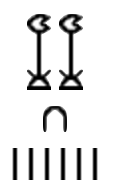
\includegraphics[width=2em]{egyptian/2016.png} \\
    \end{tabular}
\end{center}

Even so, most of the systems we are using today are positional notations\cite{knuth1998art}
because they can express infinite numbers with just a finite set of symbols called \textbf{digits}.

\subsection{Digits}

Any set of symbols can be used as digits as long as we know how to \textit{assign}
each digit to the value it represents.

\begin{center}
    \begin{adjustbox}{max width=\textwidth}
    \begin{tabular}{ | l | *{16}{l} | }
    \textbf{Numeral system} & \multicolumn{16}{c |}{\textbf{Digits} } \\
    \hline
    decimal         & 0 & 1 & 2 & 3 & 4 & 5 & 6 & 7 & 8 & 9 &    &    &    &    &    &    \\
    binary          & 0 & 1 &   &   &   &   &   &   &   &   &    &    &    &    &    &    \\
    hexadecimal     & 0 & 1 & 2 & 3 & 4 & 5 & 6 & 7 & 8 & 9 & A  & B  & C  & D  & E  & F  \\
    \hline
    \textbf{Assigned value}  & \textbf{0} & \textbf{1} & \textbf{2} & \textbf{3} & \textbf{4} & \textbf{5} & \textbf{6} & \textbf{7} & \textbf{8} & \textbf{9} & \textbf{10} & \textbf{11} & \textbf{12} & \textbf{13} & \textbf{14} & \textbf{15} \\
    \end{tabular}
    \end{adjustbox}
\end{center}

We place a bar above a digit to indicate its assignment.
Below is the assignments of hexadecimal digits.

\begin{center}
    \begin{adjustbox}{max width=\textwidth}
    \begin{tabular}{ *{4}{c} }
    $ \bar{0} \mapsto 0 $ & $ \bar{1} \mapsto 1 $ & $ \bar{2} \mapsto 2 $ & $ \bar{3} \mapsto 3 $ \\
    $ \bar{4} \mapsto 4 $ & $ \bar{5} \mapsto 5 $ & $ \bar{6} \mapsto 6 $ & $ \bar{7} \mapsto 7 $ \\
    $ \bar{8} \mapsto 8 $ & $ \bar{9} \mapsto 9 $ & $ \bar{A} \mapsto 10 $ & $ \bar{B} \mapsto 11 $ \\
    $ \bar{C} \mapsto 12 $ & $ \bar{D} \mapsto 13 $ & $ \bar{E} \mapsto 14 $ & $ \bar{F} \mapsto 15 $ \\
    \end{tabular}
    \end{adjustbox}
\end{center}

Positional numeral systems represent a number by lining up a series of digits:

$$ \xrightarrow{2016} $$

In this case, $ 6 $ is called \textit{least significant digit},
and $ 2 $ is known as the \textit{most significant digit}.
Except when writing decimal numbers,
we will write down numbers in reverse order,
from the least significant digit to the most significant digit like this

$$ \xleftarrow{6102} $$

\subsection{Syntax and Semantics}

Syntax bears no meaning;
its semantics can only be carried out by \textit{converting} to some other syntax.
Numeral systems are merely syntax.
The same notation can represent different numbers in different context.

Take the notation "11" for example; it could have several meanings.

\begin{center}
    \begin{tabular}{ | l | r | }
    \textbf{Numeral system}      & \textbf{number in decimal}  \\
    \hline
    decimal             & 11    \\
    binary              & 3     \\
    hexadecimal         & 17    \\
    \end{tabular}
\end{center}

To make things clear, we call a sequence of digits a \textbf{numeral}, or \textbf{notation};
the number it expresses a \textbf{value}, or simply a \textbf{number};
the process that converts notations to values an \textbf{evaluation}.
From now on, \textbf{numeral systems} only refer to the positional ones.
We will not concern ourselves with other kinds of numeral systems.

\subsection{Evaluating Numerals}

What we mean by a \textit{context} in the previous section is the \textbf{base} of
a numeral system.
The ubiquitous decimal numeral system as we know has the base of 10.
While the binaries that can be found in our machines nowadays has the base of 2.

\begin{center}
    \begin{adjustbox}{max width=\textwidth}
    \begin{tabular}{ | l | l | *{16}{l} | }
    \textbf{Numeral system} & \textbf{Base}  & \multicolumn{16}{c |}{\textbf{Digits} } \\
    \hline
    decimal         & 10 & 0 & 1 & 2 & 3 & 4 & 5 & 6 & 7 & 8 & 9 &    &    &    &    &    &    \\
    binary          & 2  & 0 & 1 &   &   &   &   &   &   &   &   &    &    &    &    &    &    \\
    hexadecimal     & 16 & 0 & 1 & 2 & 3 & 4 & 5 & 6 & 7 & 8 & 9 & A  & B  & C  & D  & E  & F  \\
    \hline
    \textbf{Assigned value}  & & \textbf{0} & \textbf{1} & \textbf{2} & \textbf{3} & \textbf{4} & \textbf{5} & \textbf{6} & \textbf{7} & \textbf{8} & \textbf{9} & \textbf{10} & \textbf{11} & \textbf{12} & \textbf{13} & \textbf{14} & \textbf{15} \\
    \end{tabular}
    \end{adjustbox}
\end{center}

We can see that a system would have exactly \textbf{\textit{base}} number of digits
and the assigned value of a digit ranges \textbf{from \textit{0} to \textit{base - 1}}.

Conventionally, the base of a system is annotated by subscripting it to the
right of a numeral, like $ ({2016})_{10} $.
We replace the parenthesis with a fancy pair of semantics brackets,
like $ [\![ 2016 ]\!]_{10} $ to emphasize its role as the evaluation function.

To evaluate a notation of a certain base:
$$
    [\![d_0d_1d_2...d_n]\!]_{base}
    =
    \bar{d_0}\times base^0 + \bar{d_1}\times base^1 + \bar{d_2}\times base^2 + ... + \bar{d_n}\times base^n
$$

Where $ d_{n} $ is a digit for all $ n $.

\section{Unary Numbers and Peano Numbers}

Some computer scientists and mathematicians seem to be more comfortable with
unary (base-1) numbers because they are isomorphic to the natural numbers à la Peano.

$$
    [\![1111]\!]_{1} \cong
        \overbrace{\text{suc (suc (suc (suc}}^4 + \text{ zero)))}
$$

Statements established on such construction can be proven using mathematical
induction. Moreover, people have implemented and proven a great deal of functions
and properties on these unary numbers because they are easy to work with.

However, if we are to evaluate unary numerals with the model we have just settled,
the only digit of the unary system would have to be assigned as $ 0 $ and
every numeral would evaluate to zero as a result.

We could generalize the definition of digit assignments to allow unary digits to
start counting from $ 1 $, but that would lead to inconsistency among systems
of other bases.

\begin{center}
    \begin{adjustbox}{max width=\textwidth}
    \begin{tabular}{ | l | l | *{16}{l} | }
    \textbf{Numeral system} & \textbf{Base}  & \multicolumn{16}{c |}{\textbf{Digits} } \\
    \hline
    decimal         & 10 & 0 & 1 & 2 & 3 & 4 & 5 & 6 & 7 & 8 & 9 &    &    &    &    &    &    \\
    binary          & 2  & 0 & 1 &   &   &   &   &   &   &   &   &    &    &    &    &    &    \\
    hexadecimal     & 16 & 0 & 1 & 2 & 3 & 4 & 5 & 6 & 7 & 8 & 9 & A  & B  & C  & D  & E  & F  \\
    unary           & 1  &   & 1 &   &   &   &   &   &   &   &   &    &    &    &    &    &    \\
    \hline
    \textbf{Assigned value}  & & \textbf{0} & \textbf{1} & \textbf{2} & \textbf{3} & \textbf{4} & \textbf{5} & \textbf{6} & \textbf{7} & \textbf{8} & \textbf{9} & \textbf{10} & \textbf{11} & \textbf{12} & \textbf{13} & \textbf{14} & \textbf{15} \\
    \end{tabular}
    \end{adjustbox}
\end{center}

\section{Binary Numerals in Digital Circults}

Recall how arithmetics such as long addition are performed by hand.

\begin{center}
    \begin{tabular}{c@{\,}c@{\,}c@{\,}c}
      & 1 & 2 & 3 \\
    + &   & 3 & 4 \\
    \hline
      & 1 & 5 & 7 \\
    \end{tabular}
\end{center}

The greater a number is, the longer its notation will be, which in terms
determines the time it takes to perform operations.
Since a system can only have \textbf{finitely many} digits, operations such as
addition on these digits must be \textbf{constant time}.
Consequently, the time complexity of operations such as long addition on a numeral
would be $ O(lg n) $ at best.
The choice of the base is immaterial as long as it is not unary (which would degenerate to $ O(n) $).

However, this is not the case for the binary numeral system implemented in
arithmetic logic units (ALU). These digital circuits are designed to perform fast
arithmetics. Regarding addition, it takes only \textit{constant time}.

It seems that either we have been doing long addition wrong since primary school,
or the chip manufacturers have been cheating all the time. But there's a catch!
Because we are capable of what is called \textit{arbitrary-precision arithmetic},
i.e., we could perform calculations on numbers of arbitrary size
while the binary numbers that reside in machines are bounded by the hardware,
which could only perform \textit{fixed-precision arithmetic}.

\paragraph{problem}
Judging from the time complexity of operations, the binary numerals running in
digital circuits is certainly different from the ordinary binary numerals we have
known. Moreover, the current representation of numeral system has failed to capture this.

\section{Numerical representation}

One may notice that the structure of unary numbers looks suspiciously similar
to that of lists'. Let's compare their definition in Haskell.

% use minipage for juxtaposing two blocks of codes
\noindent\begin{minipage}{.45\textwidth}
\begin{lstlisting}
data Nat = Zero
         | Suc Nat
\end{lstlisting}
\end{minipage}\hfill
\begin{minipage}{.48\textwidth}
\begin{lstlisting}
data List a = Nil
            | Cons a (List a)
\end{lstlisting}
\end{minipage}

If we replace every {\lstinline|Cons _|} with {\lstinline|Suc|} and {\lstinline|Nil|}
with {\lstinline|Zero|}, then a list becomes an unary number,
and that is precisely what the {\lstinline|length|} function,
a homomorphism from lists to unary numbers, does.

Now let's compare addition on unary numbers and merge (append) on lists:

\noindent\begin{minipage}{.48\textwidth}
\begin{lstlisting}[basicstyle=\ttfamily\scriptsize]
add : Nat → Nat → Nat
add Zero    y = y
add (Suc x) y =
    Suc (add x y)
\end{lstlisting}
\end{minipage}\hfill
\begin{minipage}{.45\textwidth}
\begin{lstlisting}[basicstyle=\ttfamily\scriptsize]
append : List a → List a → List a
append Nil         ys = ys
append (Cons x xs) ys =
    Cons x (append xs ys)
\end{lstlisting}
\end{minipage}

Aside from having virtually identical implementations, operations on unary numbers
and lists both have the same time complexity. Incrementing a unary number takes
$ O(1) $, inserting an element into a list also takes $ O(1) $; adding two unary
numbers takes $ O(n) $, appending a list to another also takes $ O(n) $.

If we look at implementations and operations of binary numbers and binomial
heaps, the resemblances are also uncanny.

[insert some images here]

The strong analogy between positional numeral systems and certain data structures
suggests that numeral systems can serve as templates for designing containers.
Such data structures are called \textbf{Numerical Representations}\cite{okasaki1996purely}
\cite{hinze1998numerical}.

A container with $ n $ elements can be modeled after the representation of the number $ n $.
These containers are composed of smaller building blocks that house elements
as numerals are composed of digits.

\paragraph{problem}
However, conventional numeral systems are incapable of modelling these numerical
representations.

[insert a table of numerical representation and their correspondense numeral systems]

\section{Outline}
The remainder of the thesis is organized as follows.
Chapter~\ref{generalizations} proposes some generalizations to accommodate the
needs of having a more versatile representation of numeral systems.
Chapter~\ref{agda} gives a introduction to \textit{Agda}, the language we use to
construct and formalize the representation.
Chapter~\ref{props} introduces \textit{equational reasoning} and relevent properties
of natural numbers used in the rest of the thesis.
Chapter~\ref{construction} constructs the representation for numeral systems and
develops properties of such representation.

% [say something about redundant data structures]

% 1. RAL {0, 1}, {1, 2}, {1, 2, 3}

% Surprisingly, we could fit these binary numbers into our representation with
% just a tweak. If we allow a system to have more digits, then a fixed-precision
% binary number can be regarded as a single digit! To illustrate this, a 32-bit
% binary number would become a single digit that ranges from $ 0 $ to $ 2^{32} $,
% while everything else including the base remains the same.
%
% Formerly in our representation, there are exactly \textit{base} number of digits
% that range from:
%
% $$
%     \text{offset}  ...  \text{offset} + \text{base} - 1
% $$
%
% We introduce a new index \textit{\#digit} to generalize the number of digits.
% Now they range from:
%
% $$
%     \text{offset}  ...  \text{offset} + \text{\#digit} - 1
% $$
%
% Here's a table of the configurations about the systems that we've addressed:
%
% \begin{center}
%     \begin{tabular}{l*{3}{r}}
%     Numeral system      & base  & \#digit    & offset    \\
%     \hline
%     Decimal             & 10    & 10        & 0         \\
%     Binary              & 2     & 2         & 0         \\
%     Unary               & 1     & 1         & 1         \\
%     Int32               & 2     & $ 2^{32} $ & 0        \\
%     \end{tabular}
% \end{center}
%
% Consider this numeral system, the oridinary binary numbers with an extra digit:
% $ 2 $.
%
% \begin{center}
%     \begin{tabular}{l*{3}{r}}
%     Numeral system      & base  & \#digit    & offset    \\
%     \hline
%     0-1-2 Binary        & 2     & 3          & 0         \\
%     \end{tabular}
% \end{center}
%
% \begin{center}
%     \begin{tabular}{c*{1}{l}}
%     Number (in decimal)  & Notation \\
%     \hline
%     0       & 0 \\
%     1       & 1 \\
%     2       & 01, 2 \\
%     3       & 11 \\
%     4       & 001, 21 \\
%     5       & 101, 12 \\
%     \end{tabular}
% \end{center}
%
% Such a numeral system is said to be \textbf{redundant}, because there are more than one
% way to represent a number. In fact, systems that allow $ 0 $ as one of the digits
% must be redundant, since we can always take a number and add leading zeros without
% changing it's value. Systems that does not have zeros are said to be \textbf{zeroless}.
%
% We will see that there's a deep connection between data
% structures and  numeral systems. Data structures modeled after redundant numeral
% systems have some interesting properties.
%
%
% % \subsubsection{From numeral systems to numbers}
%
% % But that simplicity comes at a cost, the time complexity of functions defined on
% % unary numbers is significantly
%
% % People have implemented and proven a great deal of functions and properties on
% % these unary numbers because they are easy to work with. But the simplicity comes
% % at a cost, the time complexity of functions defined on unary numbers is significantly
% % higher than those defined on systems of other bases, say, binary numbers. Hence,
% % it's not practical in doing heavy calculations.
%
% % The \textit{numbers} we are constructing in this work are the \textit{natural numbers}.
% % We learned how to count with these numbers when we are little. But what are numbers, really?
%
% % \paragraph{Recursive}
%
% % Paul Benacerraf once argued\cite{benacerraf1965numbers} that, there are two kinds
% % of \textit{counting} which corresponds to \textbf{transitive} and \textbf{intransitive}
% % uses of the verb "to count". Transitive counting, in his sense, is to assign one
% % of the numbers to the cardinality of a set, by establish a one-to-one correspondence
% % between the numbers and the objects one is counting, all the way from none to
% % all. Intransitive counting, on the other hand, is to generate a sequence of
% % notation, that could go as far as we need. And it seems that one can only learn
% % how to count intransitively first, before knowning how to count transitively,
% % but not vice versa.
% %
% % He further discussed that the numbers must be at least recursive
%
% % \paragraph{Numbers are recursive}
% %
% % \paragraph{Internal definition is immaterial}
%
\end{document}
